\documentclass[aspectratio=169,11pt]{beamer}
\usepackage{amsmath,amssymb,tikz,array}
\usetikzlibrary{arrows.meta,positioning}
\useoutertheme{miniframes}

% Match Lecture09.pdf: Computer Modern, NYU purple, narrow margins,
% section navigation, two-line footer, and lightly outlined proof states.
\definecolor{nyu}{HTML}{57068C}
\definecolor{navpurple}{HTML}{4C2A7E}
\setbeamercolor{structure}{fg=nyu}
\setbeamercolor{frametitle}{fg=nyu,bg=white}
\setbeamercolor{section in head/foot}{fg=white,bg=navpurple}
\setbeamercolor{author in head/foot}{fg=white,bg=navpurple}
\setbeamercolor{title in head/foot}{fg=white,bg=navpurple!92!black}
\setbeamercolor{normal text}{fg=black,bg=white}
\setbeamertemplate{navigation symbols}{}
\setbeamertemplate{mini frames}[default]
\setbeamersize{text margin left=3mm,text margin right=3mm}
\setbeamerfont{frametitle}{size=\large}
\setbeamerfont{section in head/foot}{size=\fontsize{6}{7}\selectfont,series=\mdseries}
\setbeamerfont{author in head/foot}{size=\fontsize{6}{7}\selectfont,series=\mdseries}
\setbeamerfont{title in head/foot}{size=\fontsize{6}{7}\selectfont,series=\mdseries}
\setbeamertemplate{footline}{%
  \begin{beamercolorbox}[wd=\paperwidth,ht=2.4mm,dp=1mm,leftskip=3mm,rightskip=3mm]{author in head/foot}%
    \usebeamerfont{author in head/foot}Jaume\hfill NYU
  \end{beamercolorbox}%
  \begin{beamercolorbox}[wd=\paperwidth,ht=2.4mm,dp=1mm,leftskip=3mm,rightskip=3mm]{title in head/foot}%
    \usebeamerfont{title in head/foot}Week 10: Metaprogramming II: Asking another computer\hfill\insertframenumber/\inserttotalframenumber
  \end{beamercolorbox}%
}
\title{Metaprogramming II: Asking another computer}
\author{Jaume de Dios Pont}
\institute{New York University}
\date{November 11, 2026}
\hypersetup{pdftitle={Week 10: Metaprogramming II: Asking another computer},pdfauthor={Jaume de Dios Pont}}

\newcommand{\code}[1]{\texttt{#1}}
\tikzset{
  proof/.style={draw=nyu!25,fill=nyu!2,inner sep=7pt,align=left},
  flow/.style={draw=black!42,semithick,-{Stealth[length=3pt,width=4pt]}},
  labeltext/.style={font=\small,text=black!65,align=center},
  purple/.style={text=nyu},
}

\begin{document}

\section{Expressions}
\begin{frame}{What is an expression?}
  Lean represents terms, including types and proofs, as trees of type \code{Expr}.

  \vspace{2mm}
  {\fontsize{8}{10}\selectfont
  \renewcommand{\arraystretch}{1.05}
  \setlength{\tabcolsep}{6pt}
  \begin{tabular}{@{}ll@{}}
    \code{inductive Expr where} & \\
    \code{\phantom{xx}| bvar\phantom{xxx} : Nat $\to$ Expr} & variable under a binder \\
    \code{\phantom{xx}| fvar\phantom{xxx} : FVarId $\to$ Expr} & local variable \\
    \code{\phantom{xx}| mvar\phantom{xxx} : MVarId $\to$ Expr} & metavariable \\
    \code{\phantom{xx}| sort\phantom{xxx} : Level $\to$ Expr} & sorts: Prop, Type, \ldots \\
    \code{\phantom{xx}| const\phantom{xx} : Name $\to$ List Level $\to$ Expr} & declared constant \\
    \code{\phantom{xx}| app\phantom{xxxx} : Expr $\to$ Expr $\to$ Expr} & function application \\
    \code{\phantom{xx}| lam\phantom{xxxx} : Name $\to$ Expr $\to$ Expr $\to$ BinderInfo $\to$ Expr} & function abstraction \\
    \code{\phantom{xx}| forallE : Name $\to$ Expr $\to$ Expr $\to$ BinderInfo $\to$ Expr} & dependent function type \\
    \code{\phantom{xx}| letE\phantom{xxx} : Name $\to$ Expr $\to$ Expr $\to$ Expr $\to$ Bool $\to$ Expr} & local definition \\
    \code{\phantom{xx}| lit\phantom{xxxx} : Literal $\to$ Expr} & number or string literal \\
    \code{\phantom{xx}| mdata\phantom{xx} : MData $\to$ Expr $\to$ Expr} & metadata around a term \\
    \code{\phantom{xx}...} &
  \end{tabular}}


  \note{First slide shown in class, at 2.2. 1 and 2.1 stay entirely in Lean.
  Start from the complete proof printed by test_constructor. Recall last week's
  arithmetic Expr datatype and explain that Lean needs a representation for
  every kind of term. These are Lean.Expr's constructor types, with argument
  names omitted. Identify each form briefly, leaving mvar for the next slide.
  Explain bound and local variables using bvar and fvar. Name the role
  of lam, forallE, sort, letE, lit, and mdata without implementing them.
  Defer de Bruijn calculations, universe arithmetic, and metadata internals.
  Return to 2.3 to inspect And, its arguments, and hp. Construct the complete And.intro proof through successive applications. closeMainGoal submits the proof expression.
  The next slide explains how an expression can represent unfinished work.
  Source: MPiL 3, Expressions,
  \url{https://leanprover-community.github.io/lean4-metaprogramming-book/main/03_expressions.html}.
  Constructor signatures checked against Lean v4.34.0-rc2, Lean/Expr.lean.}
\end{frame}

\section{Metavariables}
\begin{frame}{Metavariables: unfinished expressions}
  \code{Expr.mvar : MVarId $\to$ Expr} represents a term still to be determined.

  \vspace{4mm}
  \begin{columns}[c,onlytextwidth]
    \begin{column}{0.43\textwidth}
      \begin{center}
        \textcolor{nyu}{The goal in Lean}\\[2mm]
        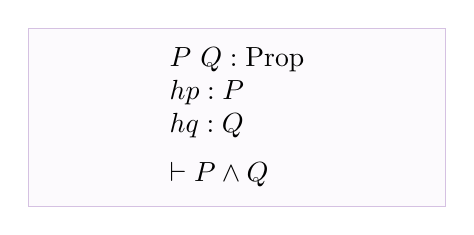
\begin{tikzpicture}
          \node[proof,minimum width=5.3cm,align=left] {
            $P\ Q : \mathrm{Prop}$\\
            $hp : P$\\
            $hq : Q$\\[2mm]
            $\vdash P \land Q$
          };
        \end{tikzpicture}
      \end{center}
    \end{column}
    \begin{column}{0.53\textwidth}
      \textcolor{nyu}{The missing proof}\\[3mm]
      {\large $\code{?g} : P \land Q$}\\[3mm]
      $\code{?g}$ is a \textbf{metavariable}:\\
      a hole in the proof expression.\\[2mm]
      Its local context includes $P$, $Q$, $hp$, and $hq$.
    \end{column}
  \end{columns}

  \vspace{4mm}
  One possible assignment is
  \quad $\code{?g} := \code{And.intro}\ hp\ hq$.

  \vspace{3mm}
  The assigned term must have the target type and use only available locals.
  \note{Use at 3.1, after the Expr slide and 2.3 inspector. Recall 2.1's goal and ask
  what term could go after the theorem's :=. Introduce ?g only after identifying
  the missing proof. Ask how the available hp can contribute to filling ?g.
  Its context determines which local terms are available.
  The displayed assignment is schematic; And.intro's implicit arguments are
  suppressed. The metavariable ID points to its type, local context, and assignment.
  Keep the construction in Lean: follow refine with named holes and use show_term
  to display the partial proof. The existential example shows a witness being
  inferred through an equality goal. The next two slides explain where the
  metavariable information lives and how an assignment is propagated.
  Source: MPiL 4, Metavariables, Overview (goals and holes in expressions),
  \url{https://leanprover-community.github.io/lean4-metaprogramming-book/main/04_metam.html}.}
\end{frame}

\begin{frame}{MetaM: context and state}
  \renewcommand{\arraystretch}{1.3}
  \setlength{\tabcolsep}{5pt}
  \begin{tabular}{@{}>{\raggedright\arraybackslash}p{3.1cm}>{\raggedright\arraybackslash}p{4.4cm}>{\raggedright\arraybackslash}p{7cm}@{}}
    & \textcolor{nyu}{Available information} & \textcolor{nyu}{What can we do?} \\[3mm]
    \textcolor{nyu}{Environment}
      & Constant declarations
      & Look up \code{Nat.succ : Nat $\to$ Nat}.\newline
        Read the body of a defined constant. \\[6mm]
    \textcolor{nyu}{Local context}
      & Variables and hypotheses in scope
      & Find the local proof \code{hp : P}.\newline
        List the available hypotheses. \\[6mm]
    \textcolor{nyu}{Metavariable context}
      & Holes: types, local contexts, and assignments
      & Create a hole \code{?x : Nat}.\newline
        Record an assignment \code{?x := 7}.
  \end{tabular}
  \note{Show at 3.2 before the recipe. Students already know monads and have seen
  constants, local variables and metavariables as Expr nodes. Use the table to
  explain what information MetaM makes available for working with those nodes.
  Recall Nat.succ and the hp lookup from 2.3, then preview the two hole operations
  in metavarDemo. The recipe slide supplies their API names and shows propagation.
  Keep withContext for 3.3 in Lean: after intro h in the two implication goals,
  ask which h the inspector should find. Explain selecting a goal's context there.
  Defer the tactic goal list to TacticM in section 4.
  Source: MPiL 4, Basic Operations and Local Contexts,
  \url{https://leanprover-community.github.io/lean4-metaprogramming-book/main/04_metam.html}.}
\end{frame}

\begin{frame}{MetaM: create, assign, instantiate}
  Build an expression containing a hole, then fill that hole.

  \vspace{3mm}
  {\small
  \renewcommand{\arraystretch}{1.55}
  \setlength{\tabcolsep}{7pt}
  \begin{tabular}{@{}lll@{}}
    \textcolor{nyu}{Step} & \textcolor{nyu}{Tool} & \textcolor{nyu}{Result} \\
    1. Create a hole & \code{mkFreshExprMVar} & Register \code{?x : Nat}. \\
    2. Build a term & \code{.app} & \code{e = Nat.succ ?x} \\
    3. Assign the hole & \code{MVarId.assign} & Record \code{?x := 7} in the context. \\
    4. Substitute its value & \code{instantiateMVars e} & Return \code{Nat.succ 7}.
  \end{tabular}}

  \vspace{3mm}
  Instantiation reads the assignment table to replace assigned holes.

  \vspace{3mm}
  The original \code{e} remains unchanged.
  \note{Run 3.2 one line at a time. After creation, inferType x reads its registered
  type. Follow the table through to instantiateMVars, which traverses e using
  the recorded assignment to replace the hole. Check e.hasMVar and filled.hasMVar
  to observe that the returned tree is new.
  Explain immutability if asked: e keeps its original tree. Computing Nat.succ 7
  to 8 is reduction; return to that operation in section 4.2.
  The assigned value must have the right type and use only the hole's allowed locals.
  mvarId! extracts the identifier of the expression returned by mkFreshExprMVar.
  In 4.2, isDefEq can infer the same assignment.
  In 5, reuse the recipe to construct And.intro with two holes. The code separately
  attaches this proof to the parent and puts the children on the tactic goal list.
  Source: MPiL 4, Basic Operations,
  \url{https://leanprover-community.github.io/lean4-metaprogramming-book/main/04_metam.html}.}
\end{frame}

\section{Elaboration}
\begin{frame}{Normal forms and definitional equality}
  \textcolor{nyu}{Which definitions may unfold? \emph{Transparency}}\\[1mm]
  {\small
  \renewcommand{\arraystretch}{1.15}
  \begin{tabular}{@{}ll@{}}
    \code{.none}      & Keep constant definitions folded. \\
    \code{.reducible} & Unfold \code{abbrev} and \code{@[reducible]} definitions. \\
    \code{.default}   & Also unfold ordinary \code{def}. \\
    \code{.all}       & Also unfold \code{@[irreducible]} definitions.
  \end{tabular}}

  \vspace{2mm}
  The same expression can have different normal forms at different transparencies.

  \vspace{2mm}
  \textcolor{nyu}{Where do we reduce?}\\[1mm]
  \code{whnf}: reduce until the outer form is exposed.\\
  Full normalisation: reduce inside arguments and function bodies too.

  \vspace{2mm}
  \textcolor{nyu}{Definitional equality (\code{isDefEq})}\\[1mm]
  Compare up to computation; may assign metavariables to make terms match.

  \note{Use with 4.2, before hypothesis in 4.3 and splitAndCore in 5.1.
  First run traceUnfolding: numberAlias, number, hiddenNumber, 7.
  Keep the operation fixed as reduceAll and change only the transparency.
  The complete hierarchy is none < reducible < instances < implicit < default < all.
  Mention the intermediate modes for instance_reducible and implicit_reducible
  definitions without a separate example.
  all does not expose opaque declarations or axioms. reduceAll does not select all
  transparency: its name refers to including implicit arguments, types and proofs.
  Next compare Both (id P) Q, And (id P) Q, and And P Q at default transparency.
  After whnf exposes And, use full reduction to enter its arguments.
  Only variables with a defining value, such as let-bound variables, can unfold.
  Both whnf and full normalisation respect transparency. WHNF is not one unfolding.
  Compare structural equality with isDefEq on the original and reduced expressions.
  Then run inferMetavar: Nat.succ ?x matches 8 by assigning x := 7.
  isDefEq also respects transparency.
  An equality requiring a theorem need not be definitional.
  Source: MPiL 4, Full Normalisation, Transparency, Weak Head Normalisation,
  Definitional Equality,
  \url{https://leanprover-community.github.io/lean4-metaprogramming-book/main/04_metam.html}.}
\end{frame}

\begin{frame}{Elaborating a term in context}
  Term elaboration turns parsed syntax into a typed expression.

  \vspace{5mm}
  \begin{center}
    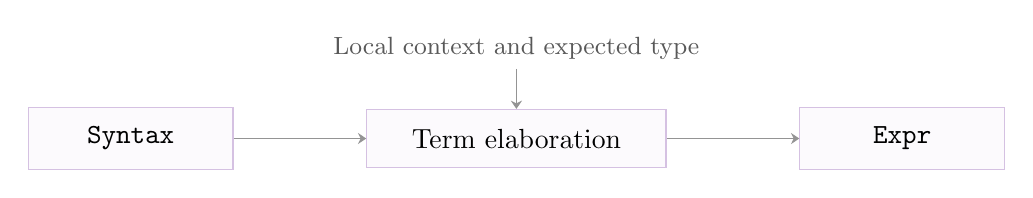
\begin{tikzpicture}[x=1cm,y=1cm]
      \node[proof,minimum width=2.6cm,align=center] (syntax) at (-4.9,0)
        {\code{Syntax}};
      \node[proof,minimum width=3.8cm,align=center] (elab) at (0,0)
        {Term elaboration};
      \node[proof,minimum width=2.6cm,align=center] (expr) at (4.9,0)
        {\code{Expr}};
      \draw[flow] (syntax) -- (elab);
      \draw[flow] (elab) -- (expr);
      \node[labeltext] (inputs) at (0,1.15) {Local context and expected type};
      \draw[flow] (inputs) -- (elab);
    \end{tikzpicture}
  \end{center}

  \vspace{3mm}
  Local names and implicit arguments are resolved using the context and expected type.

  \vspace{3mm}
  The resulting proof term must pass the kernel's type checker.
  \note{Use after the break, with 6.1--6.2. Connect to the preceding slide:
  term elaboration uses reduction and definitional equality to check types
  and solve metavariables. First elaborate n+1 in a context
  where n is unknown. If asked about evaluation, explain that elaboration resolves
  the expression and its type without computing a value for n.
  Then implement exact_term and return to 2.1's P and Q,
  hp and hq. The expected conjunction type guides the pair notation. The
  optional data pair and Int numeral show other uses of expected-type information.
  Name TermElabM here. After synthesizing pending obligations with the
  tactic-facing helper, use closeMainGoal to reject any remaining holes.
  Keep code on the Lean side. Reuse exactTerm in 9's certificate checker.
  Source: MPiL 7, Term elaboration,
  \url{https://leanprover-community.github.io/lean4-metaprogramming-book/main/07_elaboration.html};
  Olšák--Gerbscheid, my_check, as linked in README.md.}
\end{frame}

\section{External results}
\begin{frame}{Sums of squares (SOS)}
  To prove a polynomial nonnegative, write it as a sum of squares
  with nonnegative weights:
  \[
    p(\mathbf{x}) = \sum_i c_i\,q_i(\mathbf{x})^2,
    \qquad c_i \geq 0.
  \]

  For example,
  \[
    x^2+y^2+z^2-xy-yz-zx
    = \tfrac12(x-y)^2+\tfrac12(y-z)^2+\tfrac12(z-x)^2.
  \]

  \vspace{2mm}
  The weights and polynomials form a \textbf{certificate} of nonnegativity.

  \vspace{2mm}
  \begin{center}
    \textcolor{nyu}{Hard to find, easy to verify}
  \end{center}

  \vspace{2mm}
  {\small Other examples: integer factorization, satisfying assignments for SAT.}
  \note{Introduce before 7.1, in about two minutes. The variables and polynomial
  coefficients are real. Ask why the displayed identity proves nonnegativity:
  each square is nonnegative, and all three weights are 1/2.
  Ask what data another program could return: the weights and coefficients of q_i.
  This is the triangle_nonneg example in 7.2. Start the live proof with one square
  in 7.1, then build up to the weighted sum. Slide 8 connects the certificate to IO.
  The search/check contrast motivates outsourcing discovery while building the
  proof in Lean. This small identity is easy to spot; larger decompositions can
  require substantial search. This is a practical distinction, not a complexity
  lower-bound claim. SumOfSquares.py uses semidefinite programming; our adapter
  converts its numerical result into exact rational squares for the quadratic examples.
  For the other examples: multiply proposed factors, or evaluate a Boolean formula
  at a proposed assignment. These checks certify the proposed answer.
  If asked about completeness, SOS is a sufficient condition for nonnegativity.
  Source: the course's triangle_nonneg example and certificate checker; external
  search architecture inspired by leanprover/sos, \url{https://github.com/leanprover/sos}.}
\end{frame}

\begin{frame}{External search and checked evidence}
  Python calls SumOfSquares.py to find weighted squares.

  \vspace{4mm}
  \begin{center}
    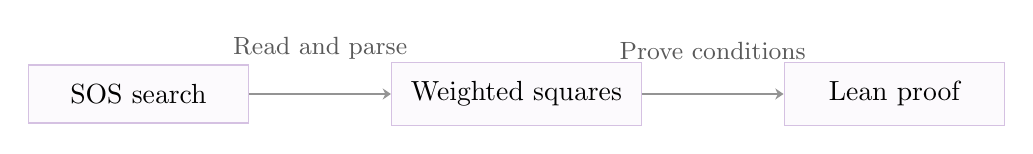
\begin{tikzpicture}[x=1cm,y=1cm]
      \node[proof,minimum width=2.8cm,align=center] (search) at (-4.8,0)
        {SOS search};
      \node[proof,minimum width=2.8cm,align=center] (data) at (0,0)
        {Weighted squares};
      \node[proof,minimum width=2.8cm,align=center] (proof) at (4.8,0)
        {Lean proof};
      \draw[flow] (search) -- node[above,labeltext,yshift=9pt]{Read and parse} (data);
      \draw[flow] (data) -- node[above,labeltext,yshift=9pt]{Prove conditions} (proof);
    \end{tikzpicture}
  \end{center}

  \vspace{4mm}
  Successful parsing establishes the response's format.

  \vspace{3mm}
  Lean checks nonnegative weights and the polynomial identity.

  \vspace{3mm}
  The IO call runs while elaborating the proof.

  \note{Use after the manual proofs in 7, across 8--12. Expose the one-square
  certificate conditions with sos_step, and solve them using split_and.
  Automate the proof with exactTerm, then extend to rationally weighted sums.
  Read the certificate from a file before calling Python. Keep the final
  five minutes for wrong weights, failed identities, and unsupported inputs.
  At those examples, explain that search failure supplies no proof for or against
  the goal: the x^4 example illustrates the limits of this search procedure.
  Show SOSProblem, add\_sos\_constraint, and solve in find\_sos.py.
  The adapter calls SumOfSquares.py with CVXOPT and uses SymPy to recover
  rational coefficients from the numerical Gram matrix. This conversion can fail.
  Use the returned coefficients to build nonnegativity proofs in Lean, then
  check their identity against the original goal with linear_combination.
  The same checker could consume certificates from a more general SOS backend.
  Sources: SumOfSquares.py, \url{https://github.com/yuanchenyang/SumOfSquares.py};
  leanprover/sos, \url{https://github.com/leanprover/sos};
  Mathlib linear_combination,
  \url{https://leanprover-community.github.io/mathlib4_docs/Mathlib/Tactic/LinearCombination.html};
  FPiL 4.5 for IO results and errors,
  \url{https://lean-lang.org/functional_programming_in_lean/Monads/The-IO-Monad/}.}
\end{frame}

\end{document}
